\documentclass[11pt]{article}
\usepackage[a4paper, portrait, margin=1in]{geometry}
\usepackage{graphicx}
\usepackage{listings}
\usepackage{epstopdf}
\usepackage{caption}
\usepackage{svg}
\usepackage{amsmath}
\usepackage{lscape}

\begin{document}

\newsavebox\IBoxA \newsavebox\IBoxB \newsavebox\IBoxC \newlength\IHeight
\newcommand\TriFig[9]{% Image1 Caption1 Label1 Image2 ...
	\sbox\IBoxA{\includegraphics[width=0.32\textwidth]{#1}}
	\sbox\IBoxB{\includegraphics[width=0.32\textwidth]{#4}}
	\sbox\IBoxC{\includegraphics[width=0.32\textwidth]{#7}}%
	\ifdim\ht\IBoxA>\ht\IBoxB
	\setlength\IHeight{\ht\IBoxB}\else\setlength\IHeight{\ht\IBoxA}\fi%
	\ifdim\ht\IBoxA>\ht\IBoxC
	\setlength\IHeight{\ht\IBoxC}\else\setlength\IHeight{\ht\IBoxA}\fi%
	\ifdim\ht\IBoxB>\ht\IBoxC
	\setlength\IHeight{\ht\IBoxC}\else\setlength\IHeight{\ht\IBoxB}\fi%  
	\begin{figure}[!htb]
		\minipage[t]{0.32\textwidth}\centering
		\includegraphics[height=\IHeight]{#1}
		\caption{#2}\label{#3}
		\endminipage\hfill
		\minipage[t]{0.32\textwidth}\centering
		\includegraphics[height=\IHeight]{#4}
		\caption{#5}\label{#6}
		\endminipage\hfill
		\minipage[t]{0.32\textwidth}\centering
		\includegraphics[height=\IHeight]{#7}
		\caption{#8}\label{#9}
		\endminipage
	\end{figure}%
}

\newcommand\TwoFig[6]{% Image1 Caption1 Label1 Image2 ...
	\sbox\IBoxA{\includegraphics[width=0.5\textwidth]{#1}}
	\sbox\IBoxB{\includegraphics[width=0.5\textwidth]{#4}}%
	\ifdim\ht\IBoxA>\ht\IBoxB
	\setlength\IHeight{\ht\IBoxB}\else\setlength\IHeight{\ht\IBoxA}\fi%
	\begin{figure}[!htb]
		\minipage[t]{0.5\textwidth}\centering
		\includegraphics[height=\IHeight]{#1}
		\caption{#2}\label{#3}
		\endminipage \hfill
		\minipage[t]{0.5\textwidth}\centering
		\includegraphics[height=\IHeight]{#4}
		\caption{#5}\label{#6}
		\endminipage
	\end{figure}%
}


\title{Advanced Systems Lab (Fall'15) -- First
Milestone}

\author{Name: \emph{Sandro Huber}\\Legi number: \emph{10-924-777}}

\date{
\vspace{4cm}
\textbf{Grading} \\
\begin{tabular}{|c|c|}
\hline  \textbf{Section} & \textbf{Points} \\ 
\hline  1.1 &  \\ 
\hline  1.2 &  \\ 
\hline  1.3 &  \\ 
\hline  2.1 &  \\ 
\hline  2.2 &  \\ 
\hline  2.3 &  \\ 
\hline  3.1 &  \\ 
\hline  3.2 &  \\ 
\hline  3.3 &  \\ 
\hline  3.4 &  \\ 
\hline  3.5 &  \\ 
\hline  3.6 &  \\ 
\hline \hline Total & \\
\hline 
\end{tabular} 
}

\maketitle

\newpage

\section{System Description}\label{sec:system-description}

\subsection{Database}\label{sec:database}

\subsubsection{Schema and Indexes}\label{sec:schema-and-indexes}
\begin{figure}[!ht]
\centering
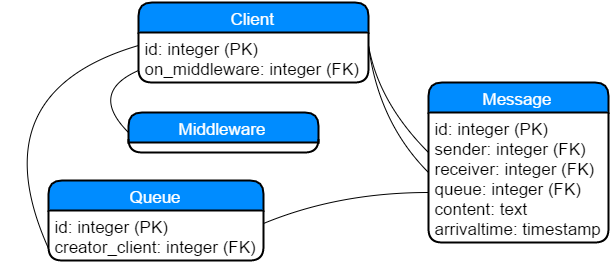
\includegraphics[width=0.6\linewidth]{figures/database/db_schema}
\caption{The Database Schema}
\label{fig:db_schema}
\end{figure}
The database schema was chosen in such a way, that it provides all required functionality, but is still easy to setup and maintain. The following lines shortly illuminate the tables and their column types.
\begin{itemize}
	\item \textbf{Client}: Guarantees through the serial datatype that each client in the whole system has a unique ID and stores which client is registered on which middleware. This can be handy when wanting an even distribution of clients over all middlewares.
	\item \textbf{Queue}: Stores all queues created by clients. Also ensures that all queues are uniquely identifiable through an ID.
	\item \textbf{Middleware}: A sequence which is used to get a unique ID for each middleware joining the system.
	\item \textbf{Message}: Here, all messages sent by clients are stored. The foreign keys ensure that we only store messages from valid clients registered in the system. As one can see, the content column is of type text, despite the choice of varchar(200) or varchar(2000) may be more obvious with respect to the system requirements. Find my thoughts about this choice in section \ref{sec:design-decisions}.
\end{itemize}
To speed up the data access I used the two following indices:
\begin{lstlisting}[language=SQL,basicstyle=\small]
(a) INDEX msg_rcvr_q_idx ON MESSAGE (RECEIVER, QUEUE);
(b) CREATE INDEX msg_sndr_idx ON MESSAGE (SENDER);
\end{lstlisting}
The reasoning behind the choice of them is based on the following thoughts. The indices in a database system affect search time, i.e. filtering of rows with respect to a criterion. Since the whole system is built with predefined stored procedures (find a full list in section \ref{sec:stored-procedures}) we know exactly what these filter parameters will be. Let's list all queries which perform some form of row selection. To simplify the view, only the most relevant parts of the individual queries are shown (query they belong to is denoted in brackets):
\begin{lstlisting}[language=SQL,basicstyle=\small,escapeinside={(*@}{@*)}]
(1) WHERE RECEIVER (*@(get\_queues\_for\_client)@*)
(2) WHERE RECEIVER AND QUEUE (*@(read\_all\_messages\_of\_queue)@*)
(3) WHERE RECEIVER AND QUEUE ORDER BY ARRIVALTIME (*@(remove\_top\_message\_from\_queue)@*)
(4) WHERE RECEIVER AND SENDER ORDER BY ARRIVALTIME (*@(read\_message\_from\_sender)@*)
\end{lstlisting}
Since an index on two columns (c1, c2) is also an index onto c1, we can see that the index (a) already covers the WHERE clauses of (1)-(3). In addition with index (b) we get a full coverage of all queries having to filter some data. It is intentional that there is no index on the GROUP BY of ARRIVALTIME. Find more about the reasoning in section \ref{sec:design-decisions}.

\subsubsection{Stored Procedures}\label{sec:stored-procedures}
Every database access is done via a stored procedure defined in the file \textit{/db\_setup/initDatabase.sql}. This allows to have a single point of failure, maintenance and control over functionality. Having this lone entry its more likely to have fast and reliable feature implementation and debugging. In Java the stored procedures are interfaced via Prepared Statments, which can be precompiled by the database, such that only the dynamic parameter values have to get fetched, before a query can be actually executed. The following stored procedures are implemented:
\begin{lstlisting}[basicstyle=\small, escapeinside={(*@}{@*)}]
create_queue(creator_client INTEGER)
delete_queue(queue_id INTEGER)
register_client(on_middleware INTEGER)
get_queues_for_client(client_receiver INTEGER)
read_all_messages_of_queue(receiver_id INTEGER, queue_id INTEGER)
read_message_from_sender(sender_id INTEGER, receiver_id INTEGER)
remove_top_message_from_queue(receiver_id INTEGER, queue_id INTEGER)
send_message(sender_id INTEGER,
	receiver_id INTEGER, queue_id INTEGER, content TEXT)
register_middleware()
get_registered_clients()
get_number_of_messages()
get_registered_queues()
take_stamp() (*@(only used by trigger take\_stamp\_trigger)@*)
\end{lstlisting}
Let's quickly look at the caller side in Java and see what happens when a stored procedure gets called (assume the procedure takes one int as input):
\begin{lstlisting}[basicstyle=\small, language=Java, showstringspaces=false]
PreparedStatement prep = myDbConnection.prepareStatement(
	"Select * from my_stored_procedure(?);");
prep.setInt(myClientID);
ResultSet rs = prep.executeQuery();
\end{lstlisting}
As one can see, the prepared statment gets actually created from a method in the (here JDBC) connection handler. This allows the database to perform the already mentionned precompilation and preoptimizations before getting confronted with the actual query call.
\subsubsection{Design decisions}\label{sec:design-decisions}
The design aims to be simple, but yet complex enough to provide all necessary functionalities through a nice interface. Please find in the following lines the reasoning about some design decision I took while implementing the system:
\begin{itemize}
	\item \textbf{text vs varchar(n)}: First of all, the datatypes char(n), varchar(n), varchar and text are internally all converted to the same C data structure varlena. So from the performance perspective no (major) differences are measurable. Because I wanted to be adaptable and send messages of length 200 and 2000 in the same setup I decided to go with the flexible choice of text. Choosing varchar(2000) so we would be able to send both, is bad, because the unused space when inserting smaller strings will be filled with spaces and thus not give any performance advantages.
	\item \textbf{Ghost-Client}: Since messages can also be addressed to all clients in the system, I introduced a ghost-client with an ID of 0, which gets created right at the database initialization. This ghost-client allows that instead of having RECEIVER=NULL, we have RECEIVER=0 for all broadcast messages, which was internally much easier and safer to handle for me.
	\item \textbf{Index on ARRIVALTIME}: Maintaining an index is not cheap for a database system, so it's wise to use them with caution. Because of that I decided that the indices (1) and (2) are already discarding enough rows, such that the sorting operation is not too costly anymore. If the database ends up to be the bottleneck, it might pay of to revisit this statement and try this nevertheless.
	\item \textbf{ARRIVALTIME location}: The ARRIVALTIME is implemented as a trigger on the database. Another, also valid choice, would have been to let the client set it. But because I wanted to minimize the work of the clients and guarantee a unique timestamp on each message I did choose the trigger-option.
\end{itemize}

\subsubsection{Performance characteristics}\label{sec:performance-characteristics}
\underline{Configuration}: To measure the performance of the database I used the postgresql tool pgbench. For the machine details, please refer to section \ref{sec:system-configurations}. I defined three levels of difficulty, which correspond to different query sets, level 0 beeing the easiest, level 2 the hardest (increasing number as well as complexity of statements). All levels are runned for 30 seconds (ignoring instable start and end seconds) for one up to 60 clients. This allows us to hopefully see a smooth transition from absolute best to real-world behaviour when benchmarking all levels. For a detailed insight into the levels, please find them in /db\_baseline/benchScripts. All contents had length 200. Before evaluating the actual database performance experiment I tested how many clients per database connection are optimal. I expected that the relation of 1:1 should hold, which indeed was the case. This makes sense, because the think-time for a client is very minimal, and thus the connection reusage very good. Even only one additional client is not worthwile. But back to our original baseline experiment.
\newline\underline{Expectation}: For the throughput and latency I expect the knee to be found around 20 clients, because we work with a machine that provides 8 physical cores and the official rule of thumb given in the PostgreSQL documentation\footnote[1]{https://wiki.postgresql.org/wiki/Number\_Of\_Database\_Connections} is \textit{optimal number of DB connections} $\approx$ $2(core\_count)+c$, where $c$ is a constant. Of course the throughput level ranking from hightest to lowest should be: 0, 1, 2+, 2- (+/- for with or without indices), and vice-versa with the latency. After the knee there should at least be a visible stagnation of the throughput, but a remarkable increase of latency.
\TwoFig {figures/database/levels0_2_tp.eps} {Database Throughput} {fig:tp}
		{figures/database/levels0_2_lat.eps} {Database Latency} {fig:lat}
\newline\underline{Reality} (figures \ref{fig:tp} and \ref{fig:lat}): Firstly please note, that the lack of data around 30 clients is explained through a bug in the code. But it does not seem that any exceptional behaviour is missed due to that. As one can see (the lines follow the 50\% quantiles), the knees can really be found around the expected 20 clients. Also the rank of the levels behave as expected. I am especially happy about the performance benefit gained by the indices. Only the gain of latency after the barely visible knee is not as steep as foreseen. But this is probably okay, since we can't see a total throughput breakdown neither.

The most costly operation in the whole benchmark is identified as the removal of the top message, i.e. executing \textit{remove\_top\_message\_from\_queue}. To further investigate this I performed the subsequent follow-up experiment.

The speed of the top most message removal is highly correlated with the size of the database, because the more messages, the longer the index access and the longer the sorting (ORDER BY) of the final table entries will take.
\newline\underline{Configuration}: To simulate an extreme scenario I only registered one client and one queue in the system into which all messages were sent. All messages also had sender and receiver set to the lone client and had a random content of length 200. This allows to focus on the behaviour of the performance of the query with respect to the size of the database. We use again the tool pgbench to realize this experiment. The database was benched by 40 concurrent clients operating on 40 database connections. I chose 40, because we just saw, that around this many clients, the database throughput on the level 2+ was maximal. Each client ran independantly and chose 3000 times randomly between either inserting 10 new messages, or removing the top most message of the single queue. This workload ensured, that the database grew over time and the whole experiment ran sufficiently long.
\newline\underline{Expectation}: As we saw in the last experiment, neither the throughput, nor the latency totally colapes or exploded. This means that we can expect here a steady increase of the latency, following the trend of the database size quite closely.
\TwoFig {figures/database/data_baseline} {Normal Configuration} {fig:data_baseline}
		{figures/database/third_index} {Extended Configuration} {fig:third_index}
\newline\underline{Reality} (figure \ref{fig:data_baseline}): It's clearly visible that the expectation of having a close relation between the performance of the query and the database size is true. To be sure, that the insertion of new messages does not blur the picture, also this data is plotted. The abrupt break-down of the latency at the end of the experiment is due to the completion of the first few clients. This allows the ones still running to get a congestion-free access to the database. The increasing variance is indicates that the query performance starts to get somewhat unstable when the database gets big enough. But nevertheless, even when going up to half a million entries in the message table, there is no extreme behaviour noticable.

\subsection{Middleware}\label{sec:middleware}

\subsubsection{Design overview}\label{sec:design-overview}
\begin{figure}[!htb]
\centering
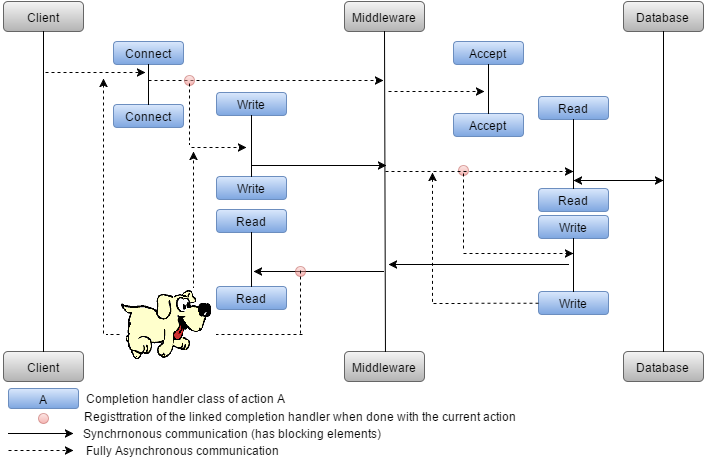
\includegraphics[width=1.0\linewidth, height=0.5\linewidth]{figures/middleware/mw_design}
\caption{A flow diagram of the whole system, showcasing the completion handler functionality. On the middleware there is a watchdog monitoring all connections, and closing them, when they were inactive for a given time interval. Yet unfinished clients would then have to reconnect.}
\label{fig:mw_design}
\end{figure}
The middleware was designed with the aim to be run fully asynchronous when communicating and be as adaptive as possible to incoming traffic. Initially I was driven by the idea of HTTP: Having a stateless protocol where each reqeust opens a new connection and closes it right after the answer is fetched. This might be nice in theory, but sadly didn't work for this type of project. Although opening a TCP socket connection is instant, closing is not. Instead of freeing the port when the connection is closed it resides in a wait state for (on windows) 30 seconds. When having around 100 clients, all sending what they can, my local system blew up around 180'000 open TCP connections, because the operating system ran out of file descriptors. That's why, the current version of the system use one TCP connection per client.

The whole project is based on the NIO-library of Java. It does allow to have a highly modular implementation with respect to the three main tasks, connection establishment, reading and writing of data. The only synchronized parts in the whole design are the sending and writing of messages, such that we can ensure that the whole request is fully sent, before returning the thread to the threadpool. Speaking of the threadpool, I did choose to work with a so called \textit{cached thread pool}. This is a dynamic, i.e unbounded thread pool, which gives the system as many threads as it needs. This is especially useful in our scenario, because we have a lot of small parallel working tasks. There is only one problem, namely deadlocks. Since in the worst case, for every read and write a blocking call is made, it's possible that all threads wait on each-other. To circumvent this, we luckily don't have to do anything. The JVM already manages a second, hidden thread pool, which takes care of all I/O operations on the asynchronous channels. This ensures, that our system is always able to react to new incoming traffic.

Let's look at a small example on how the main feature of the NIO-library, namely completion handlers, are used in case of connecting to a listening socket:
\begin{lstlisting}[basicstyle=\small, language=Java]
AsynchronousSocketChannel sc = AsynchronousSocketChannel.open();
sc.connect(inetSettings, null, new CompletionHandler<Void, Object>() {
	@Override
	public void completed(Void result, Object attachment) {
		// go here when connection successfully established
	}
	@Override
	public void failed(Throwable se, Object attachment) {
		// go here when something went wrong
	}
});
\end{lstlisting}
The nice idea here is, that the call to \textit{connect} is asynchronous. In the background, the specified completion handler is register, and whenever the contacted server socket gives an answer to our connection request, it gets executed in the \textit{cached thread pool}.
\newline\underline{Expectation}: I expect the middleware to behave stable for at least 32 concurrent clients, since we are operating with 16 hyperthreads (more machine details found in section \ref{sec:system-configurations}) and one hyperthread should surely be able to deal with two concurrent completion handlers concurrently, since the actual work done (de- and serialization, buffering, ...) is efficiently doable. Because of these thoughts, the knee should be found around 40 concurrent clients. After that, the increase of the throughput will probably slow down, and the latency itself start to increase faster.

\subsubsection{Interfacing with clients}\label{sec:interfacing-with-clients}
The interface between the clients and the middleware has two aspects: A technical and an architectural.

From the technical perspective, the interface is provided through a socket and the (IP, port)-tuples. When starting up, each client parses the IP from the console arguments provided through the calling ant script and the port number from a config file (see /config/config\_common.xml). Then the socket connection is opened and either closed by the client when it is done with it's job list, or by the watchdog operating on the middleware. The watchdog thread monitors all established connections and surveys activity among all connections in a fixed frequency of 5 seconds. If one was idle for too long it get's closed right away. Thus the client may be needed to reconnect in order to send further requests (see figure \ref{fig:mw_design}).

From an architectural point of view, the interface is given through the abstract class Request, which implements the Serializable interface. Depending on the request type of the client, a different subclass, e.g. \textit{CreateQueueRequest} is sent. The overwritten methods \textit{processOnMiddleware} and \textit{processOnClient} define the behaviour of each side for each of message. The answer sent back to the client is the same type of subclass. Just this time, the fields are set to the answers gotten from the database query. If an error happened, the \textit{exception} field is set, and thus an easy nullity test is required such that the client knows if everything went well.
The following request classes are defined:
\begin{lstlisting}[basicstyle=\small, escapeinside={(*@}{@*)}]
CreateQueueRequest
DeleteQueueRequest
GetNumberOfMessagesRequest
GetQueuesWithMessagesForClientRequest
GetRegisteredClientsRequest
GetRegisteredQueuesRequest
HandshakeRequest (*@(register a client)@*)
ReadAllMessagesOfQueueRequest
ReadMessageFromSenderRequest
RemoveTopMessageFromQueueRequest
SendMessageRequest
RegisterMiddlewareRequest
\end{lstlisting}
For every of these requests there is a corresponding exception class, which caries an informative string that explains the cause of the error, for example \textit{CreateQueueException}.

\subsubsection{Queuing and Connection pool to database}\label{sec:queuing-and-connection-pool-to-database}
When the middleware does start up, it also initializes a connection pool with open JDBC connections to the PostgreSQL database. The (IP, port)-tuple to reach the database as well as the number of concurrent database connections is again fetched from the config file found in \textit{/config/config\_common}. It's important to mention that the connections to the database are only established once in the initialization and from then on reused for the whole life of the middleware. The connection pool uses the facility of the \textit{LinkedBlockingQueue} of Java, especially the behaviour of the \textit{take} method: When there are connections available, the queue is not empty and the \textit{take} call instantly pops a connection from the queue, which will be used for the database access. If currently all connections are in use, the call to \textit{take} will block. When a connection now is returned to the pool, the \textit{LinkedBlockingQueue} internally fires a signal, which wakes a random waiting thread in the \textit{take} method up, which is allowed to proceed. This means that there is no fairness and we are not able to guarantee that a thread does not have to wait for a long time before getting a connection. Because the worst thing that can happen is, that the variance is enlarged, I decided that (as long as further experiments don't show a much worse behaviour) this is not a problem.

The queueing is implemented following the slogan \textit{'Queues are nothing, queueing is everything'}.\footnote{The orinal quote from Dwight D. Eisenhower reads \textit{'Plans are nothing, planning is everything'}. See https://en.wikipedia.org/wiki/Plan under Quotations.} Having the concept of completion handlers in hand, no explicit queue is needed. Instead, every incoming request is instantly handled by a completion handler, which also carries out the query execution. The sending of the answer is then performed by another thread of the pool, woken up by the call to the \textit{write} method in the read handler, when the database access is done.

\subsubsection{Performance characteristics}\label{sec:performance-characteristics-1}
\underline{Configuration}: To measure the performance baseline for the middleware I again tried to analyze the Unit-Under-Test as isolated as possible. In the case of the middleware this means to fully exclude the database access, but of course not the connection pooling. To generate the work load another machine, running the clients, is used. This setup of course suffers from network latency, but since we are only interested in the within-middleware response time, as long as the network bandwidth is not the bottleneck we're fine.

To verify that this is indeed true, before running the main experiment, a bandwidth measurement was done between a middleware and a client machine, which resulted in a 95\% confidence interval of $\pm15.73$MB/s $(=4.64\%)$ around $339.7MB/s$. Each measurement was performed by sending 5GB of data over the network as fast as possible. There was difference between sending the data in one big packet, or in small 1024kB blocks. This is due to the operating system which does cut the network traffic in small packets anyway. For more insight, please find the scripts for this experiment in \textit{/conn\_throughput\_baseline}. When having messages of length 200 characters, the serialized requests are $\approx2000B=2kB$ big. This means we theoretically could send $\frac{337.7MB/s}{2kB}=\frac{337700kB/s}{2kB}=168850$ requests per second. For messages of length 2000 which yield $\approx4kB$, we still can send $84425$ requests per second. Having in mind that the database level 2 maximal throughput layed at $\approx20000$ requests per second, we can be sure, that we won't have any network bottleneck when the bandwidth is that high throughout the experiments.

All requests sent in the upcoming experiment use a content size of 200, this gives us the chance to get an idea of what the best possible performance for the middleware can be.
\newline\underline{Expectation}: Because of the arguments given in section \ref{sec:design-overview} and section \ref{sec:queuing-and-connection-pool-to-database}, we can expect the system to be stable up to probably 40 clients, before the throughput breaks down and the latency increases significantly.
\TwoFig {figures/middleware/mw_throughput.eps} {Middleware Throughput} {fig:mw_tp}
{figures/middleware/mw_latency.eps} {Middleware Latency} {fig:mw_lat}
\newline\underline{Reality} (figures \ref{fig:mw_tp} and \ref{fig:mw_lat}): Let's first consider only the blue curves, i.e. the setting where the middleware was fed by a single client machine  (1CM = 1 client machine). We can clearly see, that the performance of the middleware was underestimated with respect to the number of concurrent clients that can be served while still running stable. 50 clients seem to be handled quite nicely, although the variance starts to grow now. Very strange is the sudden decrease of the troughput after 60 clients. There can be two causes for this behaviour: (1) the middleware reached it's capacity, or (2) the client is the bottleneck and too many clients are trying to send on the same client machine and hinder each other to run at full capacity. To find if (1) or (2) was the reason for this measurements I introduced a second client machine and ran the upcoming follow-up experiment.
\newline\underline{Configuration}: Let there be two client machines, which provide sending clients. Each client machine only handles half the clients with this setting. This ensures that the requests per time unit entering the middleware should at least be the same compared to the single-machine case and exceeding the old mark, where it was blocked by the limited resources available on a single machine before. 
\newline\underline{Expectation}: Peeking at the client's locale performance showed in figure \ref{fig:client_tp} (was done before this baseline), we can see that a single client machine provides $\approx$ 60'000 requests per second in a still stable manner (for a detailed experiment description see section \ref{sec:clients}). The only important fact from the client experiment is, that this performance baseline was generated by benchmarking against the simplest middleware listener possible. Since the middleware peaked at about 45'000 requests per second it seems logical to think that the middleware is really at it's limit. But this does not include the extra work the middleware has to do, namely de- and serialization and connection pooling. Let's assume this pulls the response time up to $0.03ms$. This would mean, that the clients would only be able to send $\frac{1s}{0.03ms/Req}\approx$ 33'000 requests per second. This small example shows, that it's not absurd to question the middleware as the bottleneck. So my expectation is, that the knee is pushed to the right, when splitting the work onto two client machines.
\newline\underline{Reality} (figures \ref{fig:mw_tp} and \ref{fig:mw_lat}): Now let's inspect the resulting green curves (2CM = 2 client machines). Indeed it can be verified, that the bottleneck was at the client-side. This can be said, because the throughput from 70 clients on is now stabilized with a small variance, whereas in the latter case we measured a major break-down with high instability. Having a stable throughput and simultaneously an increasing latency is a clear sign, that the performance peak of the middleware was found, in this case at around 70 clients while processing 45'000 requests per second with a response time of $\approx1$ms on average! One question the plot poses is not yet answered: Why is the throughput for two client machines lower when having less than 70 clients, compared to the single-machine case (and with the latency vice-versa)? This is indeed not so clear, and I had not enough time to investigate this further, so I can only speculate about the reasons: Having two machines, does also mean two have seperate network links. One machine probably benefits from operating system optimizations at the network layer, whereas this effect with two machines is halved. This does then lead to less throughput. But having less throughput does come with the benefit of small variance, and thus high predictability.

\subsection{Clients}\label{sec:clients}

\subsubsection{Design and interface}\label{sec:design-and-interface}
For the design please have a look at Figure \ref{fig:mw_design} again. The client is built upon the same principles as the middleware: modular, adaptive and highly parallelisable. We again use the principle of the observer pattern in combination with the completion handlers to implement the client functionality. The interface to the middlewares is provided through the already mentionned \textit{AsynchronousSocketChannel} class provided by the Java NIO-library. As explained in section \ref{sec:interfacing-with-clients}, each client fetches the IP and port number from the command line or the config file. These are then used to establish a connection to the middleware server socket channel. From then on, everything is done by the corresponding completion handlers.

\subsubsection{Instrumentation}\label{sec:instrumentation}
 To simplify the debugging a lot, I made sure that as much functionality as possible, namely accepting, writing and reading is implemented seperately. This is done by inheriting from the class \textit{CompletionHandler$<$V, A$>$} into an \textit{Accept-}, \textit{Connect-}, \textit{Read-}, and \textit{WriteCompletionHandler$<$V, A$>$}. Every client runs in its own process, so I am able to stop a certain process anytime and debug it without needing to interrupt the other ones.
 
 The logging for the benchmarks is simply done with the standard \textit{BufferedFileWriter}. I started with the log4j2 library and got it working with batched logging, but only in combination with an additional library (what is not allowed). Instead of down-grading the whole system which would have taken another day, I decided to go that way, because I had some experience in it and was able to get things running quickly. In the whole project, there are two main logging functionalities used:
 \begin{enumerate}
 	\item \textbf{Time-driven Logging}: To do this, a timer is used, that executes a scheduled logging task every x seconds. In code this looks like following:
\begin{lstlisting}[basicstyle=\small, language=Java]
myTimer.scheduleAtFixedRate(new TimerTask() {
    @Override
    public void run() {
        // write to the log file(s)
        // reset variables
    }
});
\end{lstlisting}
	\item \textbf{Event-driven Logging}: This is done by logging in the \textit{complete} method of the corresponding action. We then are sure, that this action has finished successfully.
\end{enumerate}
 
\subsubsection{Workloads and deployment}\label{sec:workloads-and-deployment}
To ensure comparable results, when not mentionned explicitly something different, I worked with a single workload that represents all important functionalities with the same weigth. The workload looks like this:
\begin{lstlisting}[basicstyle=\small,caption={Main work load},label=lst:load]
(1) Handshake
(2) Create my queue
(3) Loop until done
    (a) Send a message
    (b) Get all queues with messages waiting for me
    (c) Read all messages of one of these queues if any
    (d) Remove the top message of one of these queues if any
(4) Done when time is up or no more requests are available
\end{lstlisting}
Please note that no such thing as planned requests per second or a wait time is used to control the number of requests this workload generates. The plan is to always send as much as possible. This is useful, because we can be sure, that the client side desperately tries to flood the system with requests and nothung does hold it back in any possible way. This workload also makes sure, that the database does not grow in time. This allows making better predictions, because we can disgard one degree of freedom in the analysis. The generation of the actual requests is fully done in code. The thought behind this is, because then no file access is needed, which typically tends to be slow, the files get large fast and it's generally less flexible. The process is split into two parts:
\begin{enumerate}
	\item The client generates a list of request types (enum in class \textit{Request}). In code this looks like this:
\begin{lstlisting}[basicstyle=\small, language=Java]
RequestBuilder.addRequestTypes(
    requestList,
    new RequestType[] {
        RequestType.HANDSHAKE,
        RequestType.CREATE_QUEUE
    },
    1
);
\end{lstlisting}
This adds the array [\textit{HANDSHAKE}, \textit{CREATE\_QUEUE}] once (therefor the parameter 1) to the \textit{requestList}.
	\item When running, the client accesses this list and dynamically creates a request object of the corresponding types, passing the currently available field values (stored in a session object each client manages, where earlier answers of queries are written into) as parameters to the constructors. In code this is as simple as:
\begin{lstlisting}[basicstyle=\small, language=Java]
Request req = RequestBuilder.getRequest(
    requestList.get(reqCounter, client_session));
\end{lstlisting}, where \textit{getRequest} is simply a switch-statement over the all possible request types.
\end{enumerate}
Let's find the performance baseline for the client, generating the load described in listing \ref{lst:load}.
\newline\underline{Configuration}: The experiment conducted for this used one client and one middleware machine. As spoilered in section \ref{sec:performance-characteristics-1}, the middleware server listening here, is a minimalistic version of the one used in the real-use case. The workflow is then the following:
\begin{enumerate}
	\item The client prepares and sends a request
	\item The middleware fully reads the request
	\item The middleware instantly sends an answer, consisting of a single digit number. An answer is needed sucht the client knows when the channel is writable again.
\end{enumerate}
\underline{Expectation}: The client machine (details in section \ref{sec:system-configurations}) does provide 32 hyperthreads. Since we can assume, that the network delay in the described setting should be minimal, all of these threads should be nearly constantly busy. This means, the knee is expected to be at 32 concurrent clients for the throughput as well as the latency. To not have the client as a bottleneck it should surely be able to provide stable more than 20'000 requests per second (see database baseline performance in figure \ref{fig:tp}).
\TwoFig {figures/client/client_tp.eps} {Client Throughput behaviour} {fig:client_tp}
{figures/client/client_lat.eps} {Client Latency behaviour} {fig:client_lat}
\newline\underline{Reality} (figures \ref{fig:client_tp} and \ref{fig:client_lat}): The knee can indeed be found at 32 clients, at least for messages of length 2000. Messages of length 200 boost the maximal possible number of requests generated per second by a factor of about 1.5. The reason for that is the additional time needed for de- and serialization, and and a slightly higher network delay, simply due to package size of a single request. With 32 clients we have for both cases length 200 and 2000 a stable request generation of $\approx$45'000 requests per second.

The deployment of a client can be done in only a few steps, since the whole source code and all needed files are stored in a git repository:
\begin{enumerate}
	\item Launch a client machine and install git: \textit{sudo yum install git -y}
	\item Clone the repository to the machine: \textit{git clone https://github.com/geischtli/ASL.git}
	\item Install all needed libraries (like ant) and create necessary folders for the logging: \newline \textit{sh /home/ec2-user/ASL/client\_setup/setup\_client.sh}
	\item Start C clients on the current machine sending messages of length M to middleware with IP ADDR: \newline\textit{sh /home/ec2-user/ASL/client\_setup/start\_clients.sh -n C -m M -i ADDR}
	\item When all clients are done, simply hit \textit{ENTER} to flush and close all logging files and shutdown gracefully
\end{enumerate}

\subsubsection{Sanity checks}\label{sec:sanity-checks}
Besides the internal message counting and logging, the main sanity check is done on request level. There are two possible outcomes for a request: (1) the request is successfullly propagated through the whole system, or (2) the request is lost somewhere in between (due to a code error/bug or a network failure). In case of scenario (2) the watchdog will sometime close the TCP connection forcefully, which will lead to a thrown exception on the client side. This exception is catched and the client starts over with the request by reconnecting to the middleware. In case of scenario (1) the request is received  and deserialized by the client. It is then checked if any exception is embedded (by the middleware) in the object. If not, everything went fine. If there was an exception, the client retries the same request.

\section{Experimental Setup}\label{sec:experimental-setup}

\subsection{System Configurations}\label{sec:system-configurations}
The overall design of the system is showed in Figure \ref{fig:overall_design}. Multiple clients are launched in a single machine, but all operating in their own process. They all connect to one of the available middlewares, each running on a single machine. Each of them has a connection pool to the database. In the next sections, whenever a number of clients or connections to the database is written, please note that this number does account for the total number in the whole system. They are both shared evenly over the middlewares, if there are multiple online. For example, if 100 clients and two middlewares online and the database is accessed by 30 connections, each middleware will support 50 clients, while having a connection pool of size 15.
\begin{figure}
\centering
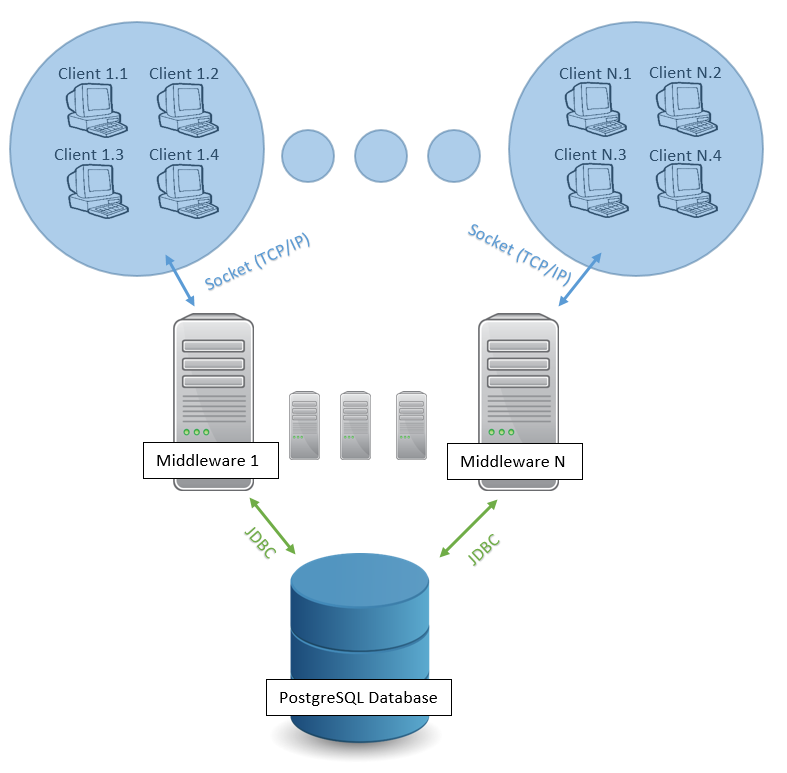
\includegraphics[width=0.5\linewidth]{figures/overall_design}
\caption{The overall system design}
\label{fig:overall_design}
\end{figure}
The detailed configurations of the machines are the following:
\begin{itemize}
	\item \textbf{Client}: The clients run on a C3.8XLarge machine. These machines provide 16 physical cores and thus allow a high number of processes to be executed concurrently.
	\item \textbf{Middleware}: The middlewares run on a C3.4XLarge machine. With their 8 physical cores they can nicely distribute the incoming read or write tasks onto the available threads.
	\item \textbf{Database}: The database runs on a R3.4XLarge machine. Besides the 8 physical cores this machine type provides, it also is equiped with 122GB of RAM. This guarantees that also big tables can still fit into the working memory.
\end{itemize}

\subsection{Configuration and Deployment mechanisms}\label{sec:configuration-and-deployment-mechanisms}
The typical experiment machine layout is setup with 2 client, 2 middleware and 1 database machine. Refering to figure \ref{fig:overall_design}, we have $N=2$. If not mentionned otherwise, the workload generated by the clients is the one, presented in listing \ref{lst:load}. The client deployment mechanism of the system was already introduced in section \ref{sec:workloads-and-deployment}. The deployment of the other two system parts follow the same schema:
\begin{itemize}
	\item \textbf{Deploy the Middleware}:
	\begin{enumerate}
		\item Enter the database IP into the corresponding field in \textit{ASL/config/config\_common.xml}
		\item Launch a middleware machine, install git and clone respository: Lookup steps (1) and (2) in section \ref{sec:workloads-and-deployment}
		\item Install all needed libraries and create necessary log folders:\newline
		\textit{sh /home/ec2-user/ASL/mw\_setup/setup\_middleware.sh}
		\item Start a middleware with a connection pool of size D on the current machine:\newline
		\textit{sh /home/ec2-user/ASL/mw\_setup/start\_middleware -d D}
		\item When the experiment is done hit ENTER to flush and close all logging files and shutdown gracefully
	\end{enumerate}
	\item \textbf{Deploy the Database}:
	\begin{enumerate}
		\item Launch a database machine and perform steps (1) and (2) of section \ref{sec:workloads-and-deployment}
		\item Setup, configure and run the database: \newline
		\textit{sh /home/ec2-user/ASL/db\_setup/setup\_database.sh}
		\item For control over the postgres process call \textit{/home/ec2-user/ASL/pg\_ctl command}, with \textit{command}, one of \{\textit{start}, \textit{stop}, \textit{status}, \textit{status}\}
		\item To setup the database quickly after the first installation use \textit{/home/ec2\_user/postgres /bin/psql -U postgres -d mydb -f /home/ec2\_user/ASL/db\_setup/initDatabase.sql}
	\end{enumerate}
\end{itemize}

\subsection{Logging and Benchmarking mechanisms}\label{sec:logging-and-benchmarking-mechanisms}
When done with the experiment it's important to fetch the data to the local machine fast and without much effort. This functionality is provided by \textit{ASL/download\_logs.sh}. Simply put the path of interest into the preconstructed command and then call it with like this: \textit{sh download\_logs.sh target\_folder}.

Sometimes the data was too big to be plotted efficiently, so I built some log parsers which do some averaging or filtering on the data. This means more work, but also that I always could go back to the original data and be sure that I have anything I need for later computations. These parsers are implemented in Java and can be found in \textit{src/org/asl/experiments/baselines /database/logParser}. When the data was ready, it was processed in Matlab where all plots are produces. The corresponding files are found in \textit{ASL/plotting tools}.

\section{Evaluation}\label{sec:evaluation}

\subsection{System Stability}\label{sec:system-stability}

\underline{Configuration}: One database, two middleware and two client machines. Each of the client machines runs 60 clients, sending and receiving messages of length 200. The workload generated by the clients is described in listing \ref{lst:load}. Each middleware handles all 60 clients of one clients machine. This made it very easy to launch the clients, because the targetted middleware IP is the same for all clients on a machine. The database was accessed through 40 concurrent connections. To run their connection pool, both middlewares got 20 of them. The database was filled with 300'000 messages to and from random clients before the experiment was run. The reason for this amount, is because, when eyeing at the database baseline with data shown in figure \ref{fig:data_baseline}, we can see that at this point the database already has a severe performance loss, but still operates stable. The database will always stay at this level of messages, because the used workload does not send more than it removes.
\newline\underline{Expectation}: Looking at all three baselines, we can easily see, that most probably the database will be the bottleneck of the whole system. Introducing an additional delay by adding a load this big, will reduce the overall throughput pretty hefty. Conretely we can try to calculate the expected outcome of the experiment:

A size 300'000 yields a remove response time of approximately $250ms$. Since all other queries are still extremely fast, they are negligible. This means a workload run through queries 3.a to 3.d also takes around $250ms$. We therefor have $\approx$16 requests per second of a single client. Now are 40 database connections open. This yields $16*40=640$ requests per second. Some of the queries are able to be executed in parallel to other queries. So let's postulate a throughput of about $16*(40+10)=800$ requests per second (assuming 10 connections can be used in parallel).
\TwoFig {figures/stability/stability_tp.eps} {Throughput behaviour} {fig:stability_tp}
		{figures/stability/stability_rt.eps} {Response time behaviour} {fig:stability_rt}
\newline\underline{Reality} (figures \ref{fig:stability_tp} and \ref{fig:stability_rt}): I'm really happy about how close the prediction was. Indeed, the only thing a bit underestimated was the parallelisability, which explains why more request could be handled than predicted. The startup of the whole system only took like 10 seconds, before it became stable. The increase at the end of figure \ref{fig:stability_tp} is explained by the reducing number of clients, since some are already finished and thus there is less congestion for the other ones. The latency does fit quite well onto the expectation: Having approximately $120ms$ per request, gives us $4*120ms=480ms$ per request package (3.a - 3.d). Of these, we know that about $250ms$ are needed for the delte operation. This yields a rest of $480-(250+10)ms=220ms$, where $10ms$ are accounted for all other network and computational work of the deletion request. Therefor the three other requests need $\approx70ms$ per request, which does not seem too bad, since the parsing of the list for example can take a lot of time when having this much messages in the system.

\subsection{System Throughput}\label{sec:system-throughput}
\underline{Configuration}: One database, two middleware and two client machines. All messages sent and received are of length 200 and stored in an empty database. The workload generated by the clients is described in listing \ref{lst:load}. This means that the size of the database (i.e. message table) will never be of remarkable size and close to 0. The obvious bottleneck in the system is currently the database. So it's important to make sure to really use this bottleneck to it's limits, in order to get a maximal throughput. Eyeing at the $2^k$ experiment performed in section \ref{sec:k-experiment}, we can see in table \ref{tbl:2k_percentages}, that the distortion between the individual factors are only small. Nevertheless we search through the scope of possible best configurations for the maximal throughput. In detail this means we run 20, 30, ... 80 each on two client machines and flood two middlewares with requests. This surely should be enough to find the maximal throughput. In detail the experiment is done by first fixing the number of connections to the database and launching the middlewares. Then the clients join the system. All 30 seconds, 10 new clients join the system. This allows us to reduce the amount of seperate runs we have to to significantly.
\newline\underline{Expectation}: We know that the throughput should maximally reach 20'000 requests per second, probably a bit less because of the network delay and the computational extra costs needed to be done at client and server side. The optimal number of database connections should be found around 40, which directly follows from the database baseline benchmark. The optimal number of clients is not so obvious to guess. I assume that it's enough as long as the clients produce enough requests, such that in addition to the middleware delay, enough requests reach the database. This is surely the case for totally 30 clients in the whole system.
\begin{figure}[!htb]
\centering
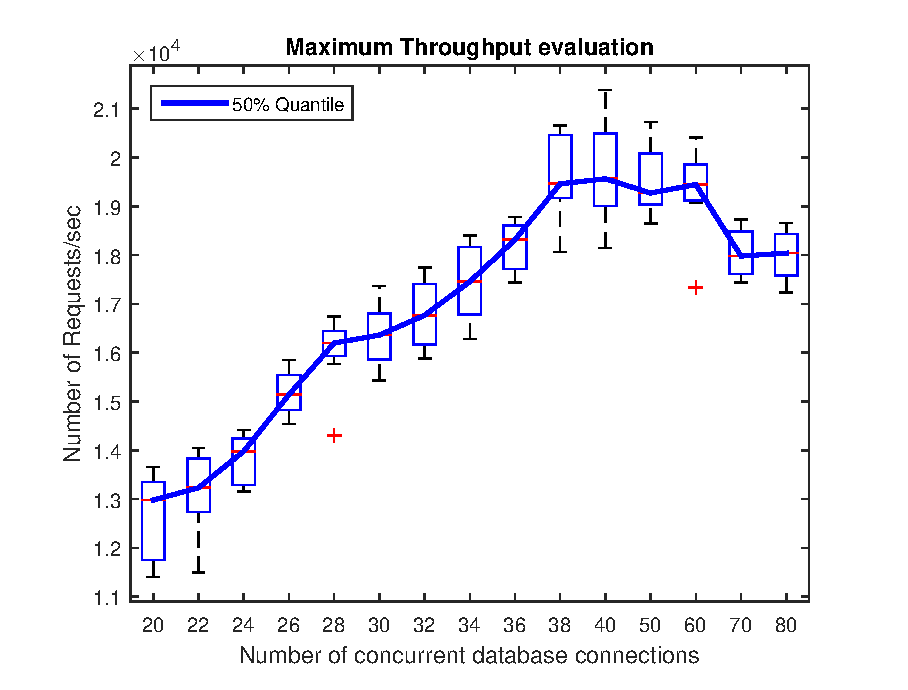
\includegraphics[width=0.7\linewidth]{figures/max_tp}
\caption{Maximum Throughput behaviour with respect to the number of database connections}
\label{fig:max_tp}
\end{figure}
\newline\underline{Reality} (figure \ref{fig:max_tp}): Pleased of the resulting plot, I can verify that the maximal throughput was indeed at approximately 19'500. The reasons for this are already given in the expectation part of this experiment. In the end, the number of clients did not make too much of a difference, when the minimally required workload could be generated. The best performance though was reached for 60 clients, 30 running on each client machine. The differences between running 30 or 60 were only minimal.

\subsection{System Scalability}\label{sec:system-scalability}

The scalability of our system is firstly watched as a question onto each seperate part of the system:
\begin{itemize}
	\item \textbf{Clients}: The client itself is easy scalable: just give it more physical resources and you're fine. Adding more clients into the system would require to have more middlewares listening.
	\item \textbf{Middleware}: The middleware itself is also only scalable through physical extendsion on machine level. Adding more middlewares only is benefitial when the other ones are oversaturated.
	\item \textbf{Database}: The database currently provides stable and reliable data access. To get scaling going one would have to introduce table and/or query optimizations.
\end{itemize}
Speaking of database optimizations, in the beginning I had the idea of introducing a third index on the column of ARRIVALTIME. Let's quickly see if it allows to scale-up the database with this modification.
\newline\underline{Configuration}: This experiment is exactly the same as already performed in section \ref{sec:performance-characteristics}. We have the isolated database machine with no middlewares or clients. 40 concurrent clients try to use 40 database connections to perform the same protocol as mentionned there. The only difference is, that now we introduce a new index, namely
\begin{lstlisting}[language=SQL,basicstyle=\small]
CREATE INDEX msg_arrtm_idx ON MESSAGE (ARRIVALTIME);
\end{lstlisting}
We again inspect the performance of the deletion, the most costly operation in the system.
\underline{Expectation}: The new index makes our search go to O(1), as soon as we have looked-up the index tree of course. The tradeoff now is that we have exact filtering, because each timestamp is unique, but the size of the index bookkeeping structures will grow immensely fast. My feeling is, that this should never pay off. Having an index this big (actually it's O(log(\#Messages)) high, when assuming a binary tree as index structure behind the scenes), the search for the right row will get extremely slow very quickly.
%\begin{figure}[!htb]
%	\centering
%	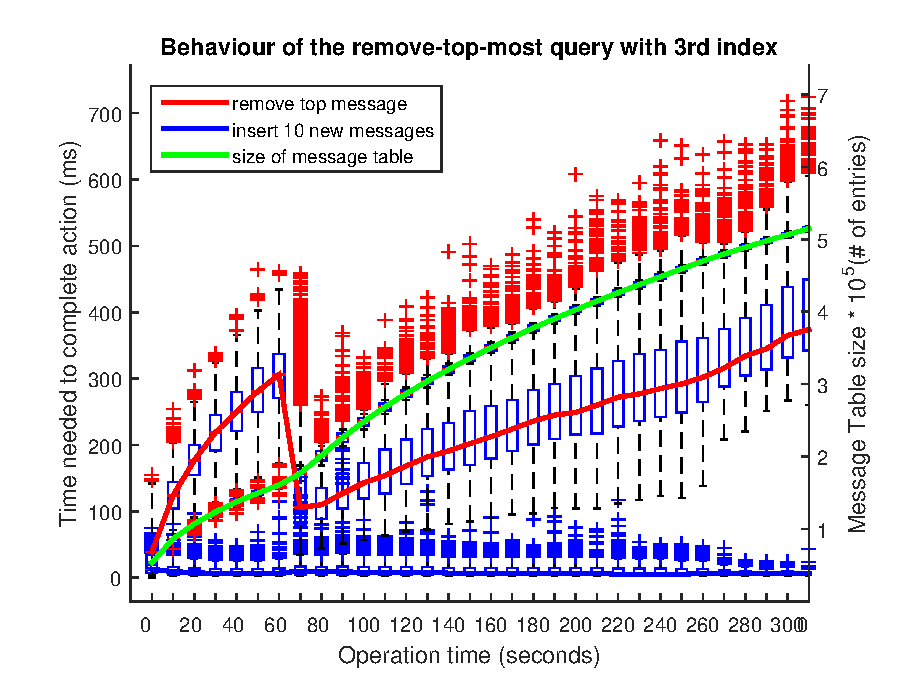
\includegraphics[width=0.7\linewidth]{figures/database/third_index}
%	\caption{}
%	\label{fig:third_index}
%\end{figure}
\newline\underline{Reality} (figure \ref{fig:third_index}): We can see that this new index really gives some problems in the early phase of the benchmark. Just to be sure this is not a random phenomena, I verified this behaviour with multiple runs. So what happens? First the index starts really to get hefty. Luckily, after 60 seconds, the automatic \textit{ANALYZE} call can safe the database from a total breakdown. The solution of it is to totally ignore the third index and only work with the two other ones. We can see that the system recovery after this repair is very fast, which is nice.

The second question related to the database is about the maximal table space, before major performance issues are recognized. So let's also try to find an answer to the scalability of the database with respect to memory.
\newline\underline{Configuration}: An entry in the message table is $4+4+4+4+200+8=224bytes$ big. Our machine amusingly is provided with exactly 224GiB of RAM. So let's add $10^9$ entries into our message table, to make sure we need more space than working memory is available. We use the same configuration as in section \ref{sec:performance-characteristics} experiment 1.
\newline\underline{Expectation}: I can't image how bad it will be, but surely the performance will drop to below a 1000 requests per second, along with a response time in the region of seconds.
\TwoFig {figures/db_scalability_1m_tp} {Throughput behaviour} {fig:tp_1m}
		{figures/db_scalability_1m_rt} {Response Time behaviour} {fig:rt_1m}
\newline\underline{Reality} (figures \ref{fig:tp_1m} and \ref{fig:rt_1m}): The throughput did really nearly completely vanish, and those clients who got some messages through had to wait for 10's of seconds. This behaviour is clear, because now, the RAM is full, and to fetch data we have to access the much slower main memory.

\subsection{Response Time Variations}\label{sec:response-time-variations}

\underline{Configuration}: This experiment was carried out under the configuration with one database, two client and one/two (depending on which line you follow in figure \ref{fig:rt_experiment}) middleware machines. There were a total of 40 concurrent database connections. The factors in this experiment are number of clients (going from 20 up 120 in total), the message size (200 or 2000) and as said, the number of middlewares (one or two). The clients did send as much as they can generating the workload described in listing 1.
\newline\underline{Expectation}: When looking at earlier benchmarks, it seems to be safe to say, that the response time for both, bigger length and more middlewares when the number of client grows should increase. Since the size of a message has indeed an inpact on the database performance, as we just saw, I assume that also here it's visible that the longer messages take a longer response time. Looking at the middleware baseline one can assume that the number of middlewares should be benefitial to the response time.
\begin{figure}[!htb]
\centering
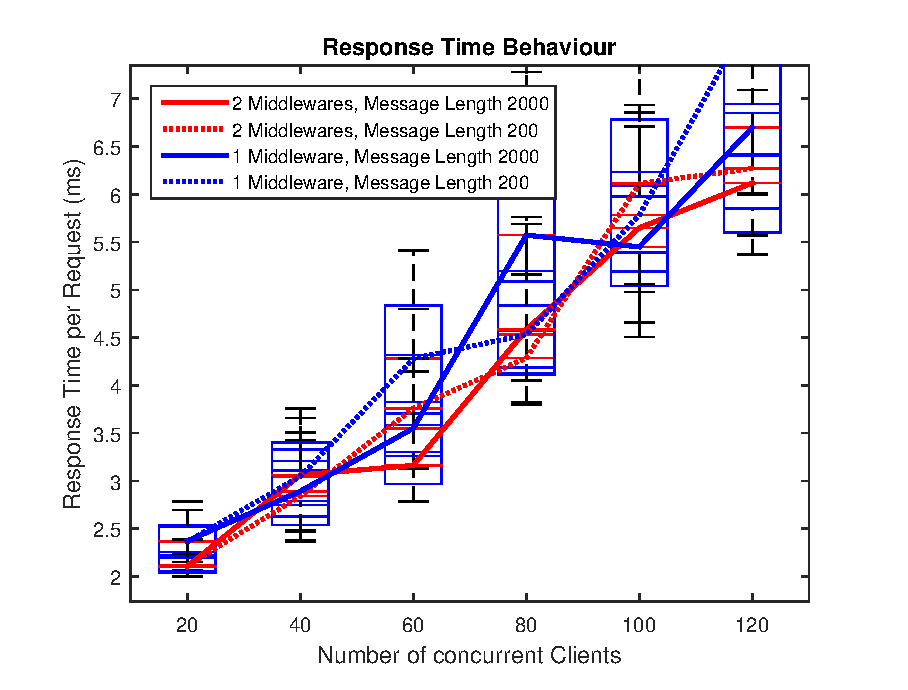
\includegraphics[width=0.7\linewidth]{figures/rt_experiment}
\caption{Respose Time Variation with respect two Middlewares, Clients and Message Size}
\label{fig:rt_experiment}
\end{figure}
\newline\underline{Reality} (figure \ref{fig:rt_experiment}): Sadly the conficence goal of 95\% was here not reached and there was nomore time to do more runs. It's therefor hard to make an exact statment, but neverteless I try. In general it seems that the expectations are met. Besides the two anomalies at 40 and 60 clients, the trends are confirmed, when also in less an explicit way. It's nice that the system seems to perform well for both configurations though.

\subsection{$2^k$ Experiment}\label{sec:k-experiment}

\underline{Configuration}: The $2^k$ experiment is performed with one database, two middleware and two client machines. The clients follow the workload schema of listing 1. The database is empty at start and will never reach a considerable size. The number of clients and number of database connections are evenly distributed over the middlewares if there are two in play. Each of the runs operated for one minute. Only the stable 30 seconds near the end are included as valid data. The runs are evaluated in terms of throughput and response time.
\newline\underline{Expectation}: After seeing the basic baselines there seem to be two factors outstanding for the performance of the system: The number of client and the connection pool size. So I expect these two to explain a lot of variance and the others much less.
\begin{landscape}
\begin{table}
\small
\centering
\caption{$2^k$ Factors}
\label{tbl:2k_labels}
\begin{tabular}{cccc}
	Symbol & Factor & Level -1 & Level 1 \\ \hline
	A & \#Middlewares & 1 & 2 \\
	B & \#Clients & 60 & 120 \\
	C & Message Length & 200 & 2000 \\
	D & \#DB Connections & 20 & 40 \\ \hline
\end{tabular}
\end{table}
\begin{table}[]
	\small
	\centering
	\caption{$2^k$ Effects}
	\label{tbl:2k}
	\begin{tabular}{|cccccccccccccccc|cc|}
		\hline
		I & A & B & C & D & AB & AC & AD & BC & BD & CD & ABC & ABD & ACD & BCD & ABCD & TP(Req/s) & RT(ms)\\ \hline
		1 & -1 & -1 & -1 & -1 & 1 & 1 & 1 & 1 & 1 & 1 & -1 & -1 & -1 & -1 & 1 & 12427 & 5.12\\
		1 & -1 & -1 & -1 & 1 & 1 & 1 & -1 & 1 & -1 & -1 & -1 & 1 & 1 & 1 & -1 & 14707 & 3.87 \\
		1 & -1 & -1 & 1 & -1 & 1 & -1 & 1 & -1 & 1 & -1 & 1 & -1 & 1 & 1 & -1 & 11859 & 4.84 \\
		1 & -1 & -1 & 1 & 1 & 1 & -1 & -1 & -1 & -1 & 1 & 1 & 1 & -1 & -1 & 1 & 16133 & 3.66 \\
		1 & -1 & 1 & -1 & -1 & -1 & 1 & 1 & -1 & -1 & 1 & 1 & 1 & -1 & 1 & -1 & 12413 & 9.98 \\
		1 & -1 & 1 & -1 & 1 & -1 & 1 & -1 & -1 & 1 & -1 & 1 & -1 & 1 & -1 & 1 & 18233 & 7.07 \\
		1 & -1 & 1 & 1 & -1 & -1 & -1 & 1 & 1 & -1 & -1 & -1 & 1 & 1 & -1 & 1 & 13238 & 9.14 \\
		1 & -1 & 1 & 1 & 1 & -1 & -1 & -1 & 1 & 1 & 1 & -1 & -1 & -1 & 1 & -1 & 16428 & 6.97 \\
		1 & 1 & -1 & -1 & -1 & -1 & -1 & -1 & 1 & 1 & 1 & 1 & 1 & 1 & -1 & -1 & 13488 & 4.69 \\
		1 & 1 & -1 & -1 & 1 & -1 & -1 & 1 & 1 & -1 & -1 & 1 & -1 & -1 & 1 & 1 & 15954 & 3.87 \\
		1 & 1 & -1 & 1 & -1 & -1 & 1 & -1 & -1 & 1 & -1 & -1 & 1 & -1 & 1 & 1 & 12289 & 4.94 \\
		1 & 1 & -1 & 1 & 1 & -1 & 1 & 1 & -1 & -1 & 1 & -1 & -1 & 1 & -1 & -1 & 15855 & 4.19 \\
		1 & 1 & 1 & -1 & -1 & 1 & -1 & -1 & -1 & -1 & 1 & -1 & -1 & 1 & 1 & 1 & 13017 & 9.16 \\
		1 & 1 & 1 & -1 & 1 & 1 & -1 & 1 & -1 & 1 & -1 & -1 & 1 & -1 & -1 & -1 & 17701 & 6.57 \\
		1 & 1 & 1 & 1 & -1 & 1 & 1 & -1 & 1 & -1 & -1 & 1 & -1 & -1 & -1 & -1 & 13054 & 9.31 \\
		1 & 1 & 1 & 1 & 1 & 1 & 1 & 1 & 1 & 1 & 1 & 1 & 1 & 1 & 1 & 1 & 12427 & 6.73 \\ \hline
		14650 & 221 & 561 & -91 & 1927 & -86 & -76 & -17 & -36 & 354 & 21 & 193 & 47 & 101 & -365 & 212 \\
		6.25 & -0.07 & 1.85 & -0.03 & -0.89 & -0.09 & 0.14 & 0.05 & -0.04 & -0.4 & 0.06 & 0.01 & -0.06 & -0.05 & 0.04 & -0.05 \\ \hline
		$q_{0}$ & $q_{A}$ & $q_{B}$ & $q_{C}$ & $q_{D}$ & $q_{AB}$ & $q_{AC}$ & $q_{AD}$ & $q_{BC}$ & $q_{BD}$ & $q_{CD}$ & $q_{ABC}$ & $q_{ABD}$ & $q_{ACD}$ & $q_{BCD}$ & $q_{ABCD}$ & 
	\end{tabular}
\end{table}
\end{landscape}

\begin{table}
\centering
\caption{Variation explained by each factor in \% (only parameters shown with values $>1\%$)}
\label{tbl:2k_percentages}
\begin{tabular}{ccc}
	Parameter & TP & RT \\ \hline
	$q_{A}$ & 1.10 & 0.12 \\
	$q_{B}$ & \textbf{7.09} & \textbf{77.57}  \\
	$q_{D}$ & \textbf{83.35} & \textbf{17.80} \\
	$q_{BD}$ & 2.82 & 3.42 \\
	$q_{CD}$ & 0.01 & 0.07  \\
	$q_{BCD}$ & 3.99 & 0.03  \\
	$q_{ABCD}$ & 1.02 & 0.05  \\
\end{tabular}
\end{table}
\underline{Reality} (table \ref{tbl:2k_percentages}): It's clearly visible, that the throughput and response time are mainly dependent of a single factor each. For the throughput, the most important factor is the number of concurrent database connections (explains $\approx83.35\%$ of the variation). For the response time however the cruial factor is the number of active clients (explains $\approx77.57\%$ of the variation). In other words this means the following:
\begin{itemize}
	\item \textbf{Throughput}: If more database connections are added, the throughput raises. If the number of database connections is reduces, also the throughput will decrease. The second important factor to consider is the number of clients operating concurrently in the whole system. With an effect of $561$ in column B (see table \ref{tbl:2k}), this yields, that when more clients join the system the throughput will go up, and vice-versa for less clients.
	\item \textbf{Response Time}: When more clients are join the system the response time will grow. If some clients leave the response time will decrease. The number of database connections has also nearly $\approx18\%$ of influence on the performance. Since the effect of $-0.89$ in the column D (see table \ref{tbl:2k}) is negative, this means, that the more connections to the database are available, the smaller the response will be, and vice-versa for less connections to the database.
\end{itemize}
\subsection{Conclusion}\label{sec:conclusion}
The system is overall performing better than I expected. It was really nice to have the Java NIO-library at hand and to make use of these amazing features. The weak spot of the system is the database. When the message stable starts to grow, the whole system performance gradually starts to decrease. I sadly had no time to investigate this issue further, besides playing with a new index, but I could imagine that a modification by e.g. introducing new tables which ease the look-up, could be benefitial in terms of throughput.

If I could start from scratch I would defenitely make use of the log4j2 library again. Logging with Java libraries is indeed quick to setup, but so much less flexible and adaptive. I would also surely stick to git as a repository manager. It's so easy and flexible and through the command line it's possible to ship the code fast and easy to multiple machines. A thing I will never do again, is to put dynamic things like the IP of the database into a config file, because I had to do a lot of git pushes just to set new IP's or ports, which gets very tiring when you have to really do a lot of experiments with a lot of machine changes.

\end{document}
